\documentclass[letterpaper,twocolumn,amsmath,amssymb,pre]{revtex4-1}
\usepackage{graphicx}% Include figure files
\usepackage{animate}
\usepackage{dcolumn}% Align table columns on decimal point
\usepackage{bm}% bold math
\usepackage{color}
\usepackage{breqn}

\newcommand{\red}[1]{{\bf \color{red} #1}}
\newcommand{\blue}[1]{{\bf \color{blue} #1}}
\newcommand{\green}[1]{{\bf \color{green} #1}}
\newcommand{\rr}{\textbf{r}}
\newcommand{\refnote}{\red{[ref]}}

\newcommand{\fixme}[1]{\red{[#1]}}

%\newcommand{\derivation}[1]{#1} % Use this to show all derivations in detail
\newcommand{\derivation}[1]{} % Use this for nice pegagogical paper...

% needsworklater is used to annotate bits that need work, but that we
% can postpone for a while.
\newcommand{\needsworklater}[1]{\emph{[#1]}}
% needsworknow is intended to prioritize stuff that needs fixing.
\newcommand{\needsworknow}[1]{\textcolor{red}{[\emph{#1}]}}

\begin{document}
\title{E Coli project paper}

%\pacs{61.20.Ne, 61.20.Gy, 61.20.Ja}
%%%%%%%%%%%%%%%%%%%%%%%%%%%%%%%%%%%%%%%%%%%%%%%%%%%%%%%%%%%%
\begin{abstract}
  This paper is about science.
\end{abstract}
\section{Introduction}
\subsection{What is the MinD system and why is it important?}
\subsection{How proteins move in cell}
\section{Methods and Initial Conditions}
The model for the behavior of the MinD and MinE proteins inside the cell
implemented the same set of 5 reaction-diffusion equations described in the paper
by Huang et al (equations 1, 2, 3, 4, and 5). A 3d grid was constructed in
cartesian coordinates with a grid spacing of .05 $\mu$m. From there, we
were able to define a cell shape on the grid, and solve the
reaction-diffusion equations numerically to observe the time evolution of
the MinD and MinE concentrations inside the cell.

Our simulation used the same diffusion constants and reaction rates as
Huang et al, which are

\begin{gather*} %format better
  \mathcal{D}_D = \mathcal{D}_{E}  = 2.5 \mu \textrm{m$^2$ / sec}, \\
  \sigma_D^{\textrm{ADP $\rightarrow$ ATP}}  = 1/\textrm{sec},  \sigma_D = 0.025 \mu \textrm{m/sec}, \\
  \sigma_{dD}  = 0.0015 \mu \textrm{m$^3$/sec}, \\
  \sigma_{de}  = 0.7/\textrm{sec}, \sigma_E = 0.093 \mu \textrm{m$^3$/sec}.
\end{gather*}

To test our computational model, we implemented a pill shaped cell, and
tested using the same cell parameters as Huang et al, which were a radius
of 0.5 $\mu$m in the middle and at the spherical endcaps, and two different
cell lengths of 4 $\mu$m and 10 $\mu$m. We found the same type of
oscillations as in their paper using these initial conditions, verifying
that our model works as intended. Below are snapshots of MinD and MinE
concentrations at 5 second timestamps in the 4 $\mu$m cell:
\newline
\newline
[insert 5 second time stamps of 4 $\mu$m sim]
\newline
\newline
We then began to define other, non-traditional cell shapes for the purpose of
modeling squished and perturbed E. coli cells, which were created
experimentally in Mannick et al. To achieve this, we went with a
cartesian lattice rather than the cylindrical lattice used in Huang et 
al's simulations, as it allows for more flexibility in defining the 
cell shape. Some of the cell shape models included a flattened pill
(stadium shape), an ellipsoid, a spherical cell, and various randomly
generated smooth shapes, such as those in the figures below. 
\newline
\newline
[insert memf print of 2-3 cell shapes]
\newline
\newline
To interpret the results, we generated several different plot views of
the printed simulation data. These plots included a time averaged view
of the protein densities in the cell; a plot tracking the location of
protein concentrations that were global maxima in space and local maxima in 
time; and an animated view that showed the actual dispersion of
protein concentrations in the cell over time. 
\subsection{Mathematical Model}
\section{Specific Results}
\subsection{Pill Shape}
\begin{figure}
  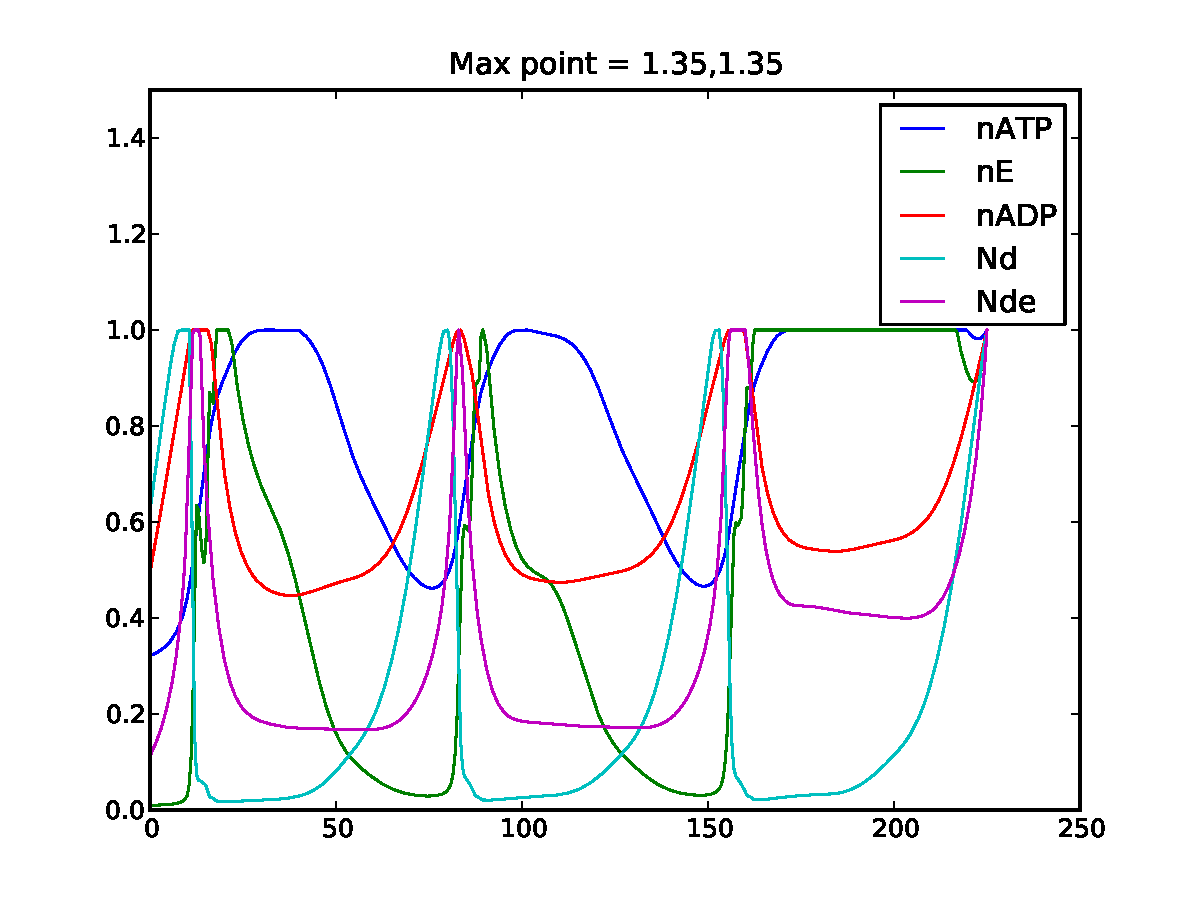
\includegraphics[width=\columnwidth]{../data/shape-p/plots/frequency_plot_all_norm-p-40-20-0-0-150.pdf}
  \caption{Protein density fluctuation with time against the polar
    wall in a 4$\mu m$ by 2$\mu m$ pill shaped cell.  The wall-bound
    proteins are shown at a point that is on the wall and the
    cytoplasm densities are shown at a point immediately adjecent.
    This plot is normalized so that every protein density peaks at 1}
  \label{frequency-plot-40-20-0-0-150}
\end{figure}

\fixme{Be more exact about what exactly Nd is versus nATP, in terms of
  the unit and dimensions.  The plotting may need to be changed}
Figure \ref{frequency-plot-40-20-0-0-150} shows the protein density
fluctuations at a point in space adjecent to a polar wall.  At each
collection of peaks the proteins reach their zenith in an order that
agrees with the qualitative picture described by
Huang\cite{huang2003dynamic}, except for nADP peak.  The peaks start
with a maxima of ATP-MinD accumulating at the walls \fixme{Need a
  better way to refer to compounds}. This peak is followed by a peak
in Nde, or ATP-MinD-MinE, as the cell is converted on the wall from
the former to the latter compound.  As this compound splits apart and
leaves the wall we see a peak in nE, or MinE in the cytoplasm.  This
is then followed by a broader peak in nATP, or the MinD-ATP compound,
as minD-ADP is (changed but I forgot the name for it) into minD-ATP in
the cytoplasm.  The minD-ATP naturally diffuses away from the pole,
which is shown by the broad nature of this peak.  All of these peaks
fit the qualitative picture except for the sharp MinD-ADP peak.  One
could except that it is a sharp peak, meaning that the MinD-ADP proteins
do not last in the cytoplasm for very long before they are converted
(once again forgot the name) into MinD-ATP.  The location of the peak
in the time dimension is troubling, however, since that we would
expect it to occur just after the peak in Nde, since the wall-bound
MinD-ATP-MinE proteins are the ones that split up and leave the wall,
creating both the MinE and the MinD-ADP.  One would expect to see the
minD-ADP peak to coincide in time with the minE peak, but it instead
coincides with the wall-bound MinD-ATP-MinE peak. (Although you can
maybe sort of convince yourself otherwiase, really looking at it).

\begin{figure}
  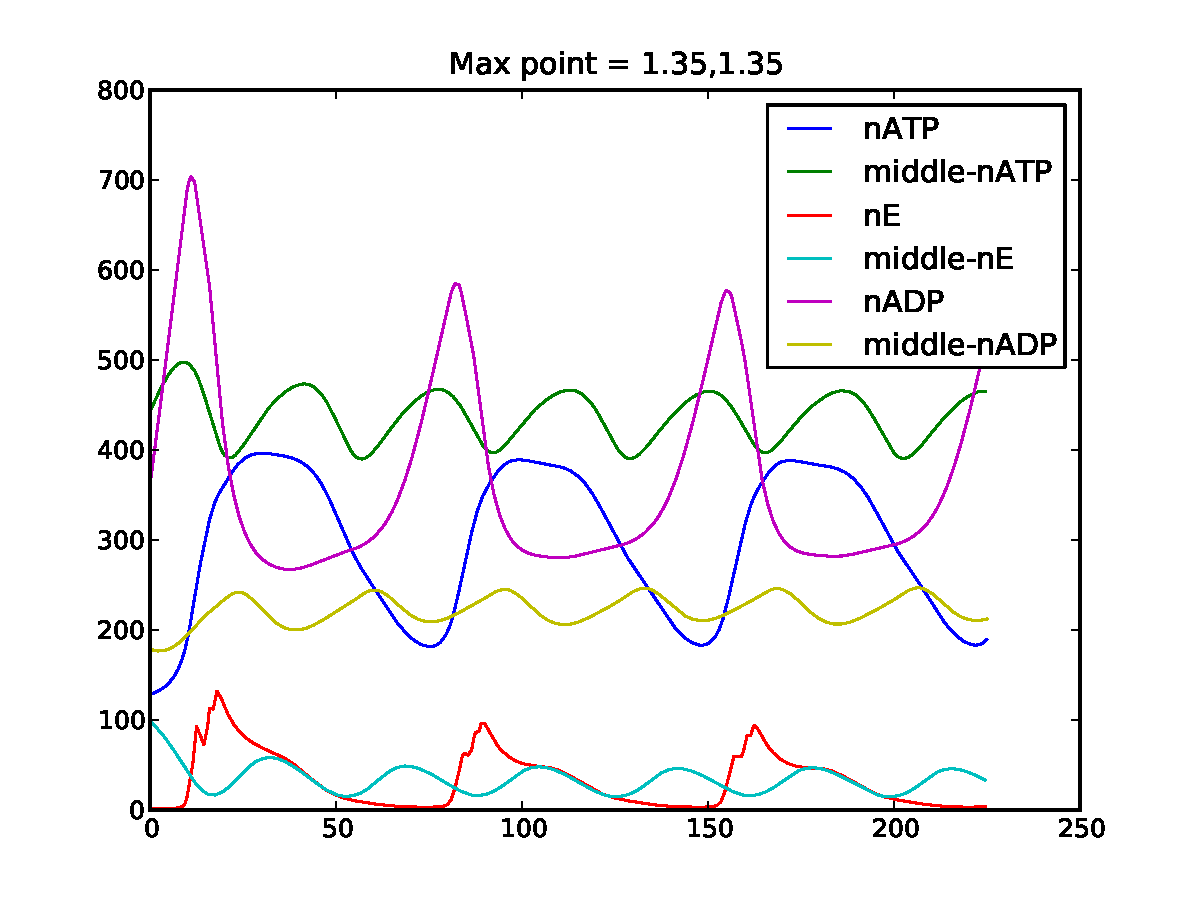
\includegraphics[width=\columnwidth]{../data/shape-p/plots/frequency_plot_all_middle-p-40-20-0-0-150.pdf}
  \caption{A comparison of protein density fluctuation with time
    against the polar wall and at a point in the center of the
    z-length and adjacent to the wall, in the cytoplasm.  The cell is
    pill shaped and has dimensions of 4$\mu m$ by 2$\mu m$.  }
  \label{frequency-plot-40-20-0-0-150}
\end{figure}

The theory states that the aversion of the FtsZ polymer to the MinC
protein is responsible for the FtsZ polymer setting up in the center
of the cell as opposed to at the cellular poles.  The MinC protein in
turn natrually associates with the minD protein that is modelled in
Huang's differential equations.  \fixme{look this up and write this
  again} The theory is dependent on there being a significant
difference in protein density between the center and polar regions. It
is worthwhile examining this difference in detail.  Figure
\ref{frequency-plot-40-20-0-0-150} shows a comparison of density
fluctuation over time at a point adjacent to the polar cell wall and
at a point adjacent to the cell wall in the center region of the cell.
The different proteins show different relationships between their
maxima and minima.  The MinD-ADP show sharp spikes at the poles and
much smaller oscillations at in the middle.  The values at the poles
are always greater than those in the middle, and the polar peaks
exhibit densities that are roughly 2.5 times greater than the maxima
in the center (\fixme{this factor and the following factor will be put
  into a table of comparisons for each protein and for the different
  cell sizes}).  The MinD-ATP densities show a very different trend.
For these it is the center density that is almost always greater than
the polar density.  The difference in density at the pole versus the
middle is a factor of roughly .85 (once again we'll do this more
officially in a table).  The MinE is similar to the MinD-ADP
comparison.  It shows a difference in maxima by a factor of roughly 2.
The MinC protein is associated with the minD protein, so perhaps the
most important camparison is between the nfl-MinD (MinD protein in all
its forms) at the ends and in the center of the pill.  This shows
sharp spikes at the pills and a maxima difference factor of roughly
1.25. \fixme{I'd like to analyze further what this means for the FtZ
  polymer.  Would a difference like this really have a big effect?
  What sort of effect should it have, looking at experimental data?
  One thing is that Mannik (is it Mannik?) genetically deletes the
  MinC protein and they get 73 percent proper cell division.  It
  really would be good to do a more extensive analysis here,
  referencing what other papers say about this.}

It would be good here to add the time map plots and discuss the idea
about the proteins spending most of their time in the center of the
cell.

Figure \ref{frequency-plot-40-20-0-0-150} also shows that the middle
density oscillates at a frequency that is twice that of the polar
regions, which is to be expected considering the symmetry of the
center compared to the that of the polar regions.  Also, the
difference between density maxima and minima each oscillation is
smaller for the middle points than for the polar points.  This is
evident from simply watching the simulation movies - the fluctulations
are more extreme in the polar regions.

Add a table here that shows the period of oscillations versus the cell
dimensions.  Do the mathematical solution of the differential
equations for an infinite long cylinder with different widths to see
how fast the mxima move and compare (Dr. Roundy says that making the
radial speed infinite would help.


\subsection{Randst shape}
\subsubsection{Randst-96-Star}
\subsubsection{Randst-97-}
\subsubsection{Randst-98-Actually Random}
\subsubsection{Randst-99}
\section{Interpretation of Data}
\section{Conclusion}
\section*{Appendix}
\bibliography{paper}











%%Below are NOTES for the Writing













\section{Introduction}
It is vital during the process of bacterial cell division for proper nucleiod occlusion that the FtsZ polymer chain develop on the cell wall in the center of the cell.  Huang et all have shown in simulation that a system of Min protein interaction within the cell will lead to a natural oscillation of the MinC protein from one cell end to the other that will leave the center free of any build up of MinC.  This will allow for the PtsZ chain to develop in the center and not at the ends, where the two nucleiods are housed.  The interaction takes place between MinE,MinD, and MinC, which naturally associates with MinD.
They gneetically mutate the bacterial cells in order to eliminate certain proteins from them.  They eliminate MinC and SlmA.  SlmA deletion has very little effect accept for some assymetry in cell division area.  The MinC deletion shows a difference in volume division.  Only 73 percent divide with the approximate 1:1 ratio while for un deleted 99 percent do.This effect is seen in both flattened and unflattened cells, and its very similar in both, which is suprising.
Mannik et all have shown that the formation of irregular cell shapes adversly effects the Min system's ability to maintain their regular oscillatory behavior.  They use microfabricated silicon chips that have etched microchambers and shallow channels.

\subsection{What is the MinD system and why is it important?}


-Systm of proteins in E.Coli and other cells.
-Theorized to be instrumental in cell citokenisis. Reference experiments
\subsection{How proteins move in cell}
-Reference experimental showing proteins oscillating
-Reference theory showing difEQ model shows oscillations
-Reference Mannik shoving into crevices.
-Worthwhile studying effect of walls shape on the movement of cells
(Sign post of what to expect from this paper)

\section{Methods and Initial Conditions}
\subsection{Mathematical Model} %shouldn't be a scripty mu
The model for the behavior of the MinD and MinE proteins inside the cell
implemented the same set of 5 reaction-diffusion equations described in the paper
by Huang et al (equations 1, 2, 3, 4, and 5). A 3d grid was constructed in
cartesian coordinates with a grid spacing of .05 $\mu$m. From there, we
were able to define a cell shape on the grid, and solve the
reaction-diffusion equations numerically to observe the time evolution of
the MinD and MinE concentrations inside the cell.

Our simulation used the same diffusion constants and reaction rates as
Huang et al, which are

\begin{gather*} %format better
  \mathcal{D}_D = \mathcal{D}_{E}  = 2.5 \mu \textrm{m$^2$ / sec}, \\
  \sigma_D^{\textrm{ADP $\rightarrow$ ATP}}  = 1/\textrm{sec},  \sigma_D = 0.025 \mu \textrm{m/sec}, \\
  \sigma_{dD}  = 0.0015 \mu \textrm{m$^3$/sec}, \\
  \sigma_{de}  = 0.7/\textrm{sec}, \sigma_E = 0.093 \mu \textrm{m$^3$/sec}.
\end{gather*}

To test our computational model, we implemented a pill shaped cell, and
tested using the same cell parameters as Huang et al, which were a radius
of 0.5 $\mu$m in the middle and at the spherical endcaps, and two different
cell lengths of 4 $\mu$m and 10 $\mu$m. We found the same type of
oscillations as in their paper using these initial conditions, verifying
that our model works as intended. Below are snapshots of MinD and MinE
concentrations at 5 second timestamps in the 4 $\mu$m cell:
\newline
\newline
[insert 5 second time stamps of 4 $\mu$m sim]
\newline
\newline
We then began to define other, non-traditional cell shapes for the purpose of
modeling squished and perturbed E. coli cells, which were created
experimentally in Mannick et al. To achieve this, we went with a
cartesian lattice rather than the cylindrical lattice used in Huang et 
al's simulations, as it allows for more flexibility in defining the 
cell shape. Some of the cell shape models included a flattened pill
(stadium shape), an ellipsoid, a spherical cell, and various randomly
generated smooth shapes, such as those in the figures below. 
\newline
\newline
[insert memf print of 2-3 cell shapes]
\newline
\newline
To interpret the results, we generated several different plot views of
the printed simulation data. These plots included a time averaged view
of the protein densities in the cell; a plot tracking the location of
protein concentrations that were global maxima in space and local maxima in 
time; and an animated view that showed the actual dispersion of
protein concentrations in the cell over time. 
\section{Specific Results}
%-Datahjhuj and plots that show concrete results. Pill normal is for the establishing that we have what works, reference  other paper, then modify, is the idea.
\section{Pill Shape}
Pill Normal section - 
Our goal with this project was to test whether or not the computational model developed by
Huang et al was consistent with the newer experimental results (squishing E
Coli) produced by Mannick et al. We generally see that:

- Protein concentrations bounce around to areas with high curvature.
- - example: nflD randst 1 6 6 99 tri-polar zones with tri-polar concentrations
- - nflE the same
- There is some time delay between where different protein types appear.



The pills with larger cylindrical widths, 4.00 3.00 (the wider pill shapes)
exhibit oscillations with maxima reached on either side (half period
times) 30s, 70s, 110s, so first half oscillation occured in 30s, the
next two in 40s

The 4.00 2.00 pills exhibit a similar pattern, but max out at times
25s,55s,85s,115s, so thirty seconds each half period.  Seemed once again that
the first oscillation had a higher max density, then settled down.  I
wonder if extremely increasing the starting condition density
lopsidedness will still yield a settle down pattern with the same max
densities?  Is this dependent on shape/size?

The 4.00 0.50 pill seemed to show oscillations of 20 second half
periods very consistently.  Density maximum did not seem to lose
intensity.  Seemed to be the same each oscillation.

 Also with this, when look at the periods and max
denisty/min density ratio, consider the size dimensions of the pill
shape and see if can see a mathematical relation.

The nflE 4.00 0.50 shows a very large difference in center highest density
versus pole highest density (during a maxima).  Is this perhaps the
protein that's more important.

Looking at the extrema plots - one very interesting thing is the 4.00
2.00 ATP extrema, which shows the extrema only in the center of the
cell.  The other proteins for this shape show the extrema to be at the
ends.  Also, it seems the 4.00 3.00 cell shapes for these plots are
missing.  Very interesting to see if there is a certain protein that
has its maxima in the center of the cell, while the others have maxima
elsewhere.  Tells a story that could maybe relate to the other shapes.

Also, try starting the cells with density only in the corner.  Now the
extrema go down the center of the cell, see if there would remain a
lopsided nature of the oscillations if you started it like this instead.

The very long cells have very long periods

The time map plots seem inconsistent in that some show the highest
densities on the poles, some in the centers, some on just one pole.
For these want to run starting from a time when the proteins are
evenly spread out (so between two maxima) and stop at a similar pointe
at the end.

The time map plots that I believe though sometimes show that the max
density time-wise is actually in the middle of the cell!  Make sure we
have a good, longer view of this being true.


Important


Pill Short -
     -Know how short is too short

Randst 99 -

\section{Randst shape}
whats the difference between the extremes in density at different
places (like the density max at the poles and at the rims in the
center).  Still need to do this.

There are sudden bursts in the nflE protein plots, at the poles. Their
density maxima build very quickly then diffuse more slowly.

\subsection{randst-96}
The star shape (randst-96) Shows oscillations in nflD horizontally,
two poles to two poles.  There is sometimes a small amount of lag
between the upper maxima moving horizontally and the lower.  Half
periods take roughly 25s. Dimensions are roughly 5.00 by 5.00?  Check
this.  The nflE short bursts do develop lag between when the top and
the bottom go off.  Should coordinate this with the nflD lag.

Tried to see if there is a time correlation between nflE and nflD but
the maxima seem to appear in the poles at roughly the same time.

Watched Nd and nE simulations next to each other at same time.  Both
have maxima that build up right at the walls (in the corners) and then
subside.  It's clear that the nE density bursts appear directly after
the Nd bursts.  The Nd bursts are subsiding as the nE bursts are
rising up.  The Nd reaches a time maxima just before the nE.  This is
true in each corner, so that when the maxima are lopsided top to
bottom - when the top right corner maximizes first, say, the interplay
between nE and Nd remains very clear in those corners where and when
maxima occur.

Watched nATP and nADP together.  nATP maxima seem to follow slightly
after nADP maxima.  This is not surprising since in rotation nATP
follows after nADP.  nATP maxima is more spread out - inbetween pole
maxima there is more spread out maxima in the center.  This should
show itself in the time map plotting.  About this - the percentage
difference seem to be the same between the non-max places and max
places, roughly, its just that the nATP seems to have a max region
that covers a wider area throughout the oscillation (or at least in
between the maxima points in the oscillation).

Also watched the Nd next to the nATP.  The Nd maximize more extreme in
the corners up against the walls.  The nATP density follows the Nd
maxima, it looks like the nATP maxima follows the Nd.  So if the Nd
appears somewhere (in a corner) then the nATP will travel there to
follow.


\subsection{randst-97}
Randst 97 nflE starts with small maxima, not much difference at all,
then actually builds to high maxima at the poles.
\subsection{randst-99}
Randst 99 (sort of triangle) is roughly dimensions of 3.5 by 3.5?
nflD oscillations appear to be half periods of 25s as well.  Maxima appear
at the poles and in the interim there are weak maxima in center pole.
\subsection{randst-98}
Funny randst shape 98 shows nflD oscillations of about 30s or so.

nADP and nATP side by side.  nADP maximizes in the corners right
before the nATP maxima follows.  Makes sense looking at equations.
Once again the nATP maxima is more spread out, where maxima in nADP
appear more just at walls.

Nd and nATP side by side.  Nd maximizes at walls and the nATP moves in
to follow it

Nd and nE side by side.  Nd maximizes in corners and then the nE also
maximizes in the corners.  The nE maxima appear in these sort of quick
bursts in the corners, along with a slower broader movements away from
that corner after the burst and into the next, where another sharp
burst occurs.  The Nd bursts occurs after the Nd as subsided in that
corner, and really by the time the burst maximizes, the Nd is already
on its way over and starting to build on the otehr side.

Randst nflD doesn't show much oscillation at all, but we start it so
that the density is not max at the pole.






%%\begin{figure}
%%   \includegraphics[width=\columnwidth]{../data/shape-randst/plots/time-map-compare-randst-10-80-60-980-150.pdf}
%%   \caption{randst 98}
%%   %\label{fig:pair-distribution-3}
%% \end{figure}
%% \begin{figure}
%%   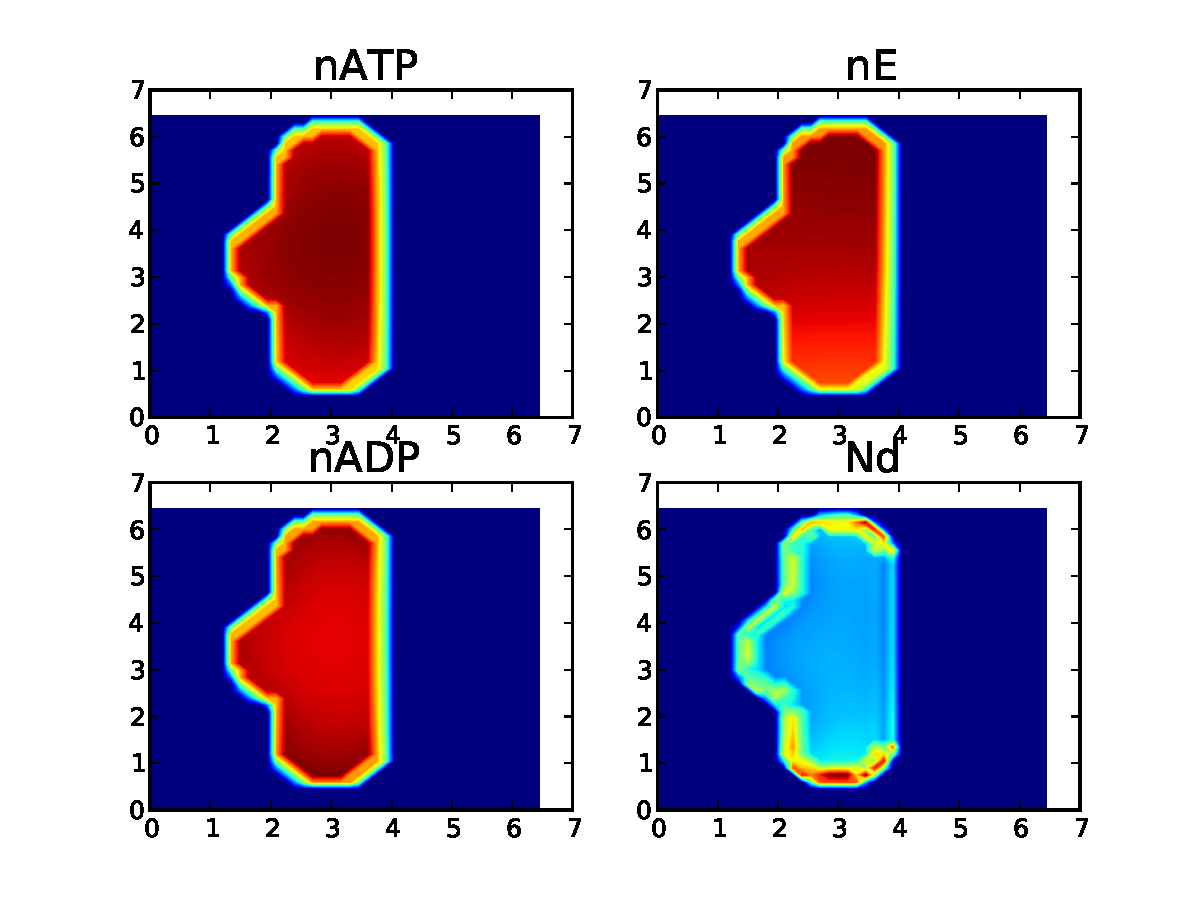
\includegraphics[width=\columnwidth]{../data/shape-randst/plots/time-map-compare-randst-10-60-60-970-150.pdf}
%%   \caption{randst 97}
%%   %\label{fig:pair-distribution-3}
%% \end{figure}
%% \begin{figure}
%%   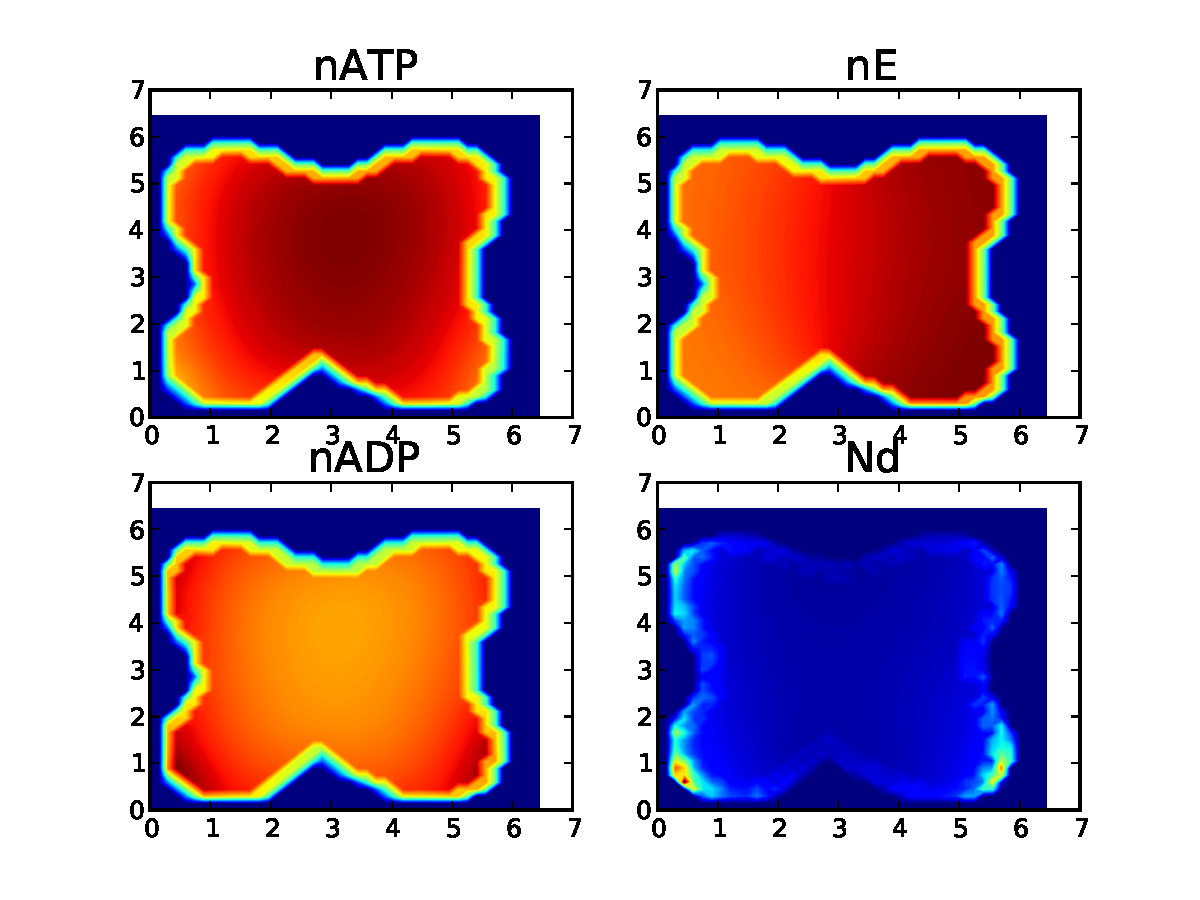
\includegraphics[width=\columnwidth]{../data/shape-randst/plots/time-map-compare-randst-10-60-60-960-150.pdf}
%%   \caption{randst 96}
%%   %\label{fig:pair-distribution-3}
%% \end{figure}

Randst 98 -

Randst 97 -

Randst 96 -

Triangle -


\section{Interpretation of Data}
-Discussion of conceptual reasons of why we see what we see
-Plots that are more interpretive (area-rating)
-Some sort of predictive claim?

\section{animate?}
\animategraphics[height=2.8in,autoplay,controls]{12}{../data/shape-randst/plots/movie-density-Nd-96/animate_}{0}{120}



\section{Conclusion}



\end{document}
